\documentclass[14pt, professionalfont]{article}

\usepackage{amssymb, amsfonts, amsthm}
\usepackage[fleqn]{amsmath}
\usepackage[dvipsnames]{xcolor}
\usepackage[many]{tcolorbox}
\usepackage{fancyhdr}
\usepackage{atbegshi}
\usepackage[hidelinks]{hyperref}
\usepackage{float}
\usepackage[left=0.18\paperwidth, right=0.18\paperwidth, top=0.12\paperheight, bottom=0.18\paperheight]{geometry}


\usepackage{graphicx}
\usepackage{framed}
\usepackage{hyperref}

\usepackage[perpage]{footmisc}
\usepackage{wrapfig}
\usepackage{subcaption}
\usepackage{booktabs}
\usepackage{tabu}

\usepackage{xepersian}
\settextfont{IRLotus}
\setdigitfont{IRLotus}
\setlatintextfont{Tom's New Roman}

\renewcommand{\baselinestretch}{1.15} 
\setlength{\mathindent}{0pt}
\setcounter{secnumdepth}{4}
\setcounter{tocdepth}{4}
\hypersetup{
	colorlinks=false,
	pdfborder={0 0 0},
}

\title{ پروژه۲ سیستم های مخابرات 
	}
\author{دکتر صباغیان}
\date{نیم سال اول 98-99 }

\makeatletter
\let\thetitle\@title
\let\theauthor\@author
\let\thedate\@date
\makeatother

\pagestyle{fancy}
\fancyhf{}
\rhead{\theauthor}
\lhead{\thetitle}
\cfoot{\thepage}

\newcommand{\E}{\text{$\mathbb{E}$}}
\renewcommand{\P}{\text{$\mathbb{P}$}}

\begin{document}	
\begin{titlepage}
	\centering
	\vspace*{2 cm}
	\begin{minipage}{\textwidth}
		\begin{minipage}{0.5\textwidth}
			\flushright
			
\includegraphics[scale = 0.55]{ece.png}
			\vspace*{0.5 cm}
		\end{minipage}
		\begin{minipage}{0.5\textwidth}
			\flushleft
			
\includegraphics[scale = 0.30]{ut.png}
			\vspace*{0.5 cm}
		\end{minipage}		
	\end{minipage}
	
	\textsc{\LARGE دانشکده فنی دانشگاه تهران}\\[0.5 cm]
	\textsc{\Large دانشکده برق و کامپیوتر}\\[0.5 cm]
	\rule{\linewidth}{0.2 mm}
	{ \LARGE  \bfseries \vspace{5pt} \thetitle}\\
	\vspace{5 pt}
	{\LARGE
		\lr{Analog modulation}}
	
	\rule{\linewidth}{0.2 mm} \\[1.5 cm]
	\begin{minipage}{0.2\textwidth}
		\begin{flushright} \large
			\emph{طراح:}\\
			\rl{سجاد پاکدامن ساوجی}
			
		\end{flushright}
	\end{minipage}~
	\begin{minipage}{0.3\textwidth}
		\begin{flushleft} \large
			\emph{رایانامه} \\
			\lr{sj.pakdaman@ut.ac.ir}
		\end{flushleft}
	\end{minipage}\\[2 cm]
	{\large \thedate}\\[2 cm]
	\vfill
\end{titlepage}
	
	{ \Large
		
		دانشجویان عزیز، قبل از پاسخ‌گوئی به سوالات به نکات زیر توجه کنید:
		\begin{enumerate}
			\item 
			شما باید کدها و گزارش خود را با الگو
			\:
			\lr{CA2\_StudentNumber.zip}
			\:
			در محل تعیین شده آپلود کنید
			\item 
			گزارش کار شما نیز جزو معیار های ارزیابی خواهد بود در نتیجه زمان کافی	 برای تکمیل آن اختصاص دهید
			\item 
			
			قسمت اصلی کد شما باید در محیط 
			\:
			\lr{matlab live editor}
			\:
			نوشته شود و نمودار ها علاوه‌ بر گزارش کار باید در کد اصلی نیز قرار داشته باشند

			\item 
			شما میتوانید سوالات خود را از طریق ایمیل
			\textcolor{blue}{
				\: 
				\href{mailto:sj.pakdaman@ut.ac.ir}{sj.pakdaman@ut.ac.ir}
				\:}
			بپرسید
		\end{enumerate}
	}
	
	\thispagestyle{empty}
	\clearpage
	\pagenumbering{arabic} 
	\pagebreak
	در این تمرین کامپیوتری به شبیه سازی مدولاسیون های آنالوگ دامنه ، فاز و فرکانس می‌پردازیم. همچنین روش های مختلف دمدولاسیون و خطای ناشی از اختلاف فرکانس کار در فرستنده و گیرنده را بررسی می‌کنیم.
	
	
	\begin{enumerate}
		\item 
		در طول این تمرین می‌خواهیم سیگنال پیام شکل ۱ را با روش های مختلف مدوله کنیم. از سیگنال پیام در بازه
		$[-1,1]$
		 با 
		$f_s = 600$
		نمونه برداری کنید. سیگنال حاصل و تبدیل فوریه آن را رسم کنید. (نمودار حوزه زمان باید برحسب ثانیه و نمودار حوزه فرکانس بر حسب 
		$Hz$
		باشد
		)
		
		\begin{minipage}[c]{0.45\textwidth}
				\begin{figure}[H]
				\centering
				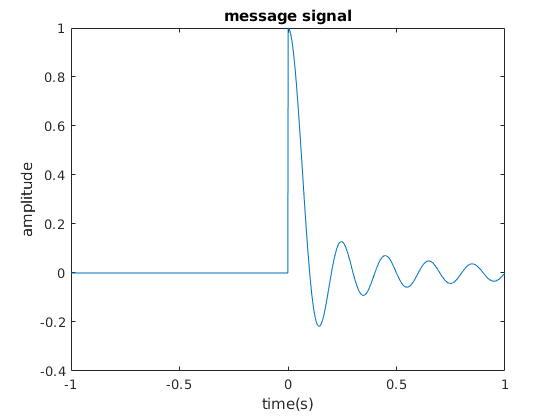
\includegraphics[scale = 0.25]{../images/message.png}
				\caption{
					سیگنال
					$m(t)$
				}
			\end{figure}
		\end{minipage}
		\begin{minipage}[c]{0.5\textwidth}
			$x_m(t) = \begin{cases}
				sinc(10t) \qquad 0 \leq t \leq 1\\
				0 \qquad \qquad \qquad o.w
			\end{cases}$
		\end{minipage}
	\item 
	ساده ترین نوع مدولاسیون دامنه ، 
	\:
	\lr{Conventional AM}
	\:
	است.
	$x_c(t) = A_c\left(1+ \mu x_m(t)\right)cos 2\pi f_c t\qquad \qquad$
	
	
	تابعی بنویسید که سیگنال پیام 
	\:
	$x_m(t)$
	\:
	،دامنه موج حامل 
	\:
	$A_c$
	\:
	،اندیس مدولاسیون 
	\:
	$\mu$
	\:
	و فرکانس موج حامل 
	\:
	$f_c$
	\:
	را ورودی بگیرد و سیگنال مدوله شده را باز گرداند. تابع را در حالت کلی پیاده‌سازی کنید تا برای هر ورودی عملیات مدولاسیون را بدرستی انجام دهد.
	\begin{enumerate}
		\item
		سیگنال پیام را با فرکانس های 
		$f_c = \{10,50,100\}$
		مدوله کنید و سیگنال‌های مدوله شده را رسم نمایید. همچنین سیگنال پیام را با فرکانس های 
		$f_c = \{600 , 1200\}$
		مدوله کنید و سیگنال‌های مدوله شده را رسم نمایید. بالا ترین فرکانس موج حامل که قابل استفاده می‌باشد چه مقداری است؟‌
		\item 
		پیام را با 
		\:
		$f_c = 100 Hz$
		\:
		مدوله کنید و تبدیل فوریه سیگنال مدوله شده را بر حسب 
		$Hz$
		رسم کنید. 
		\item 
		تابعی بنویسید که سیگنال مدوله شده 
		\:
		$x_c(t)$
		\:
		،دامنه موج حامل 
		\:
		$A_c$
		\:
		،اندیس مدولاسیون 
		\:
		$\mu$
		\:
		و فرکانس موج حامل 
		\:
		$f_c$
		\:
		را ورودی بگیرد و سیگنال پیام را از آن استخراج کند. برای دمدولاسیون پیام می‌توانید از دیاگرام شکل ۲ استفاده کنید. در نرم‌افزار متلب برای اعمال فیلتر پایین گذر می‌توانید از تابع 
		\:
		\lr{lowpass()}
		\:
		استفاده کنید. 
		\begin{figure}[h]
			\centering
			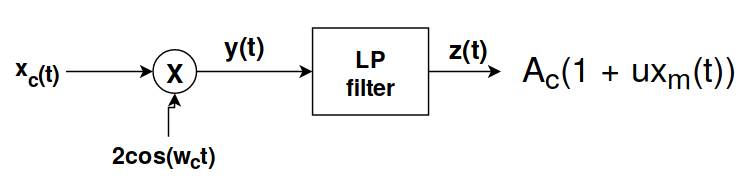
\includegraphics[scale = 0.25]{../images/amdemod.png}
			\caption{
				دیاگرام دمدولاسیون برای 
				\lr{Conventional AM}
			}
		\end{figure}
		\item 
		سیگنال های
		\:
		$y(t)$
		\:
		و 
		\:
		$z(t)$
		\:
		در شکل ۲ را در حوزه زمان و فرکانس رسم نمایید. سیگنال‌های  
	دمودله شده
		و
		\:
		$x_m(t)$
		\: را در یک نمودار رسم نمایید و  با استفاده از معیار میانگین مجذور خطا
		\:
		\lr{MSE}
		\:
		اختلاف آن‌ها را بدست آورید. 
		\item 
		اندیس مدولاسیون 
		\:
		$\mu$
		\:
		و فرکانس موج حامل 
		\:
		$f_c$
		\:
		هایپر پارامتر های این مدولاسیون هستند ،‌به عبارت دیگر این پارامتر ها را باید از قبل تعیین کرد. یکی از معیار‌های مناسب برای انتخاب این پارامتر ها مقدار اختلاف سیگنال دمدوله شده با سیگنال پیام اولیه است. نمودار خطا 
		\:
		\lr{MSE}
		\:
		نسبت به اندیس مدولاسیون
		\:
		$\mu = [-4,4]$
		\:
		را رسم کنید و توضیح دهید بهترین انتخاب برای 
		\:
		$\mu$
		\:
		چیست.
		\item 
		نمودار خطا 
		\:
		\lr{MSE}
		\:
		نسبت به فرکانس موج حامل
		\:
		$f_c = [-500 , +500]$
		\:
		را رسم کنید و توضیح دهید بهترین انتخاب برای 
		\:
		$f_c$
		\:
		چیست. 
	\end{enumerate}
	
	
	
	
	\item
	مدولاسیون بعدی که پیاده سازی می‌کنیم 
	\:
	\lr{DSB}
	\:
	است.
	$x_c(t) = A_c x_m(t) cos 2\pi f_c t\qquad \qquad \qquad \qquad \qquad$
	
	تابعی بنویسید که سیگنال پیام 
	\:
	$x_m(t)$
	\:
	،دامنه موج حامل 
	\:
	$A_c$
	\:
	و فرکانس موج حامل 
	\:
	$f_c$
	\:
	را ورودی بگیرد و سیگنال مدوله شده را باز گرداند.
	\begin{enumerate}
		\item
		سیگنال پیام را با فرکانس های 
		$f_c = \{10,50,100\}$
		مدوله کنید و سیگنال‌های مدوله شده را رسم نمایید. همچنین سیگنال پیام را با فرکانس های 
		$f_c = \{600 , 1200\}$
		مدوله کنید و سیگنال‌های مدوله شده را رسم نمایید. بالاترین فرکانس موج حامل که قابل استفاده می‌باشد چه مقداری است؟‌
		\item 
		
		$f_c = 100 Hz$
		\:
		مدوله کنید و تبدیل فوریه سیگنال مدوله شده را بر حسب 
		$Hz$
		رسم کنید.
		\item 
		به جای طراحی مدولاتور جدید برای مدولاسیون 
		\:
		\lr{DSB}
		\:
		می‌توان مطابق شکل ۳ از دو مدولاتور 
		\:
		\lr{Conventional AM}
		\:
		استفاده کرد. سیگنال پیام را با فرکانس موج حامل  
		\:
		$f_c = 100 Hz$
		\:
		به روش شکل ۳ مدوله کنید و اختلاف سیگنال مدوله شده را با سیگنال مدوله شده در قسمت قبل با معیار 
		\:
		\lr{MSE}
		\:
		بدست آورید.
			\begin{figure}[h]
			\centering
			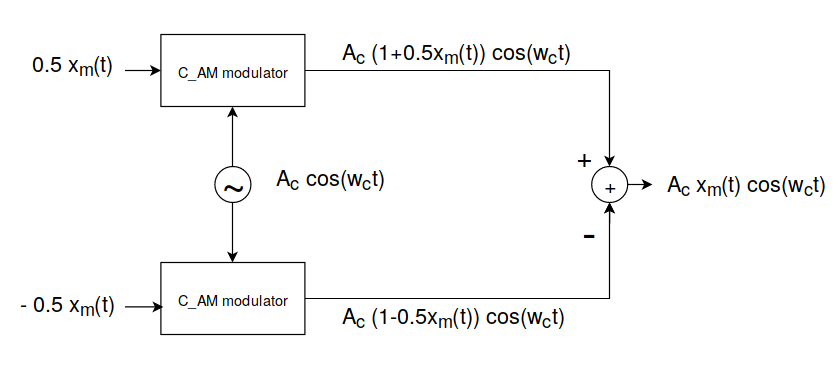
\includegraphics[scale = 0.25]{../images/dsb2am.png}
			\caption{دیاگرام مدولاسیون
				\:\lr{DSB}\:
				با استفاده از 
				\:\lr{Conventional AM}}
		\end{figure}
		\item
		تابعی بنویسید که سیگنال مدوله شده 
		\:
		$x_c(t)$
		\:
		،دامنه موج حامل 
		\:
		$A_c$
		\:
		و فرکانس موج حامل 
		\:
		$f_c$
		\:
		را ورودی بگیرد و سیگنال پیام را از آن استخراج کند. برای دمدولاسیون پیام می‌توانید از دیاگرام شکل ۴ استفاده کنید. در نرم‌افزار متلب برای اعمال فیلتر پایین گذر می‌توانید از تابع 
		\:
		\lr{lowpass()}
		\:
		استفاده کنید. 
		\begin{figure}[h]
			\centering
			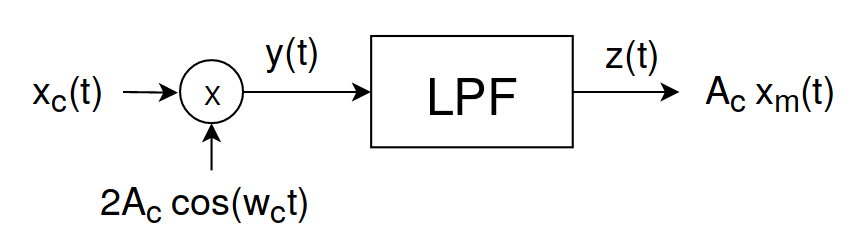
\includegraphics[scale = 0.25]{../images/dsbdemod.png}
			\caption{
				دیاگرام دمدولاسیون برای 
				\lr{DSB}
			}
		\end{figure}
		
	\item 
	سیگنال های
	\:
	$y(t)$
	\:
	و 
	\:
	$z(t)$
	\:
	در شکل ۴ را در حوزه زمان و فرکانس رسم نمایید. پیام استخراج شده
	و
	\:
	$x_m(t)$
	\: را در یک نمودار رسم نمایید و  با استفاده از معیار میانگین مجزور خطا
	\:
	\lr{MSE}
	\:
	اختلاف آن‌ها را بدست آورید.
	\item
	نمودار خطا 
	\:
	\lr{MSE}
	\:
	نسبت به فرکانس موج حامل
	\:
	$f_c = [-500 , +500]$
	\:
	را رسم کنید و توضیح دهید بهترین انتخاب برای هایپر پارامتر 
	\:
	$f_c$
	\:
	چیست.
	
	\end{enumerate}
	\pagebreak
		\item
		مدولاسیون 
		\:
		\lr{SSB}
		\:
		از چه نظر به مدولاسیون 
		\:
		\lr{DSB}
		\:
		برتری دارد؟
		\begin{equation*}
			x_c(t) = \frac{A_c}{2} \left(x_m(t)\cos w_c t - \hat{x}(t)\sin w_ct\right) \qquad USSB
		\end{equation*}
		\begin{equation*}
		x_c(t) = \frac{A_c}{2} \left(x_m(t)\cos w_c t + \hat{x}(t)\sin w_ct\right) \qquad LSSB
		\end{equation*}
		برای هر‌یک از مدولاسیون‌های فوق تابعی بنویسید که سیگنال پیام 
		\:
		$x_m(t)$
		\:
		،دامنه موج حامل 
		\:
		$A_c$
		\:
		و فرکانس موج حامل 
		\:
		$f_c$
		\:
		را ورودی بگیرد و سیگنال مدوله شده را باز گرداند. برای اعمال تبدیل هیلبرت می‌توانید از تابع 
		\:
		\lr{hilbert()}
		\:
		استفاده کنید. 
		 سپس قسمت های زیر را برای هر‌دو مدولاسیون انجام دهید :
		\begin{enumerate}
			\item 
			سیگنال پیام را با فرکانس موج‌حامل 
			\:
			$f_c = 100Hz$
			\:
			مدوله کنید و سیگنال مدوله‌شده را در حوزه رمان و فرکانس رسم نمایید.
			\item
			برای دمدولاسیون های 
			\:
			\lr{SSB}
			\:
			می‌توان از دمدولاتور 
			\:
			\lr{DSB}
			\:
			مطابق شکل ۵ استفاده کرد. سیگنال مدوله شده در قسمت قبل را دمدوله کنید و با استفاده از معیار 
			\:
			\lr{MSE}
			\:
			اختلاف پیام استخراج شده و پیام اصلی را بیابید. همچنین سیگنال های 
			\:
			$y(t)$
			\:
			و
			\:
			$z(t)$
			\:
			را در حوزه زمان و فرکانس نمایش دهید.
			\begin{figure}[h]
				\centering
				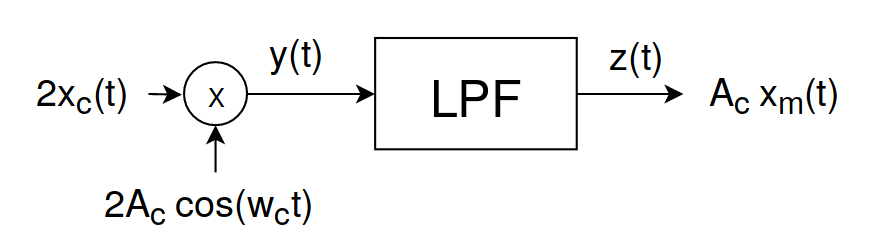
\includegraphics[scale = 0.25]{../images/ssbdemod.png}
				\caption{
					دیاگرام دمدولاسیون برای 
					\lr{SSB}
				}
			\end{figure}
		\end{enumerate}
	\item 
	در قسمت های قبل برای استخراج پیام از سیگنال مدوله شده از دمدولاتور های سنکرون استفاده کردیم. یکی از چالش های پیاده سازی سیستم های سنکرون همگام سازی فرکانس در گیرنده و فرستنده است.  برای هر یک از مدولاسیون های 
	\:
	\lr{Conventional AM}
	\:
	،
	\:
	\lr{DSB}
	\:
	،
	\:
	\lr{USSB}
	\:
	و
	\:
	\lr{LSBB}
	\:
	مراحل زیر را انجام دهید :
	\begin{enumerate}
		\item 
		سیگنال پیام را با 
		\:
		$f_c = 100 Hz$
		\:
		مدوله کنید و در گیرنده سنکرون با 
		\:
		$f^{'} = f_c \pm 0.01 f_c$
		\:
		پیام را استخراج کنید. پیام استخراج شده و پیام اصلی را در حوزه زمان در یک نمودار رسم  نمایید. 
		\item
		در حالت کلی پیام در فرستنده با فرکانس 
		\:
		$f_c$
		\:
		مدوله می‌شود و در گیرنده با فرکانس 
		\:
		$f_c \pm \Delta f$
		\:
		استخراج می‌شود . نمودار 
		\:
		\lr{MSE}
		\:
		پیام اصلی و پیام استخراج شده را بر حسب 
		\:
		$\Delta f = [-50 , 50]$
		\:
		برای 
		\:
		$f_c = 100 Hz$
		\:
		رسم نمایید.
		
	\end{enumerate}
با توجه به نتایج بدست آمده کدام‌یک از مدولاسیون ها در مقابل نوسانات فرکانس مقاوم تر است؟
\item 
(امتیازی) مراحل سوال ۵ را برای مدولاسیون های 
\:
\lr{PM}
\:
و
\:
\lr{FM}
\:
 انجام دهید.
 با توجه به نتایج بدست آمده ،‌ از بین مدولاسیون های دامنه و فرکانس کدام‌یک حساسیت کم‌تری نسبت به نوسانات فرکانس دارند؟
	\end{enumerate}
\end{document}